% =============================================================================
% Part II, Chapter 10: Cohorts 024, 025, and 025.1
% =============================================================================
\chapter{The 21-Arm Cross-Lineage Quantization Matrix and Archive Re-Audits (Cohorts 024, 025, and 025.1)}\label{ch:cohorts_024_025}

Between November 16 and November 19, 2026, Project CausalFade executed its largest multi-model quantization study---Cohort~024, comprising \textbf{$30{,}912$ scheduled LLM inference requests} ($64.1\%$ of all LLM calls in the entire project!) across three independent 7B--8B transformer lineages and all seven standard GGUF precision tiers---followed by two zero-inference cross-cohort mathematical audits (Cohorts~025 and 025.1). If post-training quantization selectively degraded causal confounding resistance relative to matched noncausal controls across open-weight instruction models, Cohort~024 was engineered to see it. Instead, Cohort~024 delivered a sweeping empirical refutation of naive cross-precision causal benchmarking (Figure~\ref{fig:c24_matrix} and Table~\ref{tab:c24_matrix}).

\begin{figure}[htbp]
  \centering
  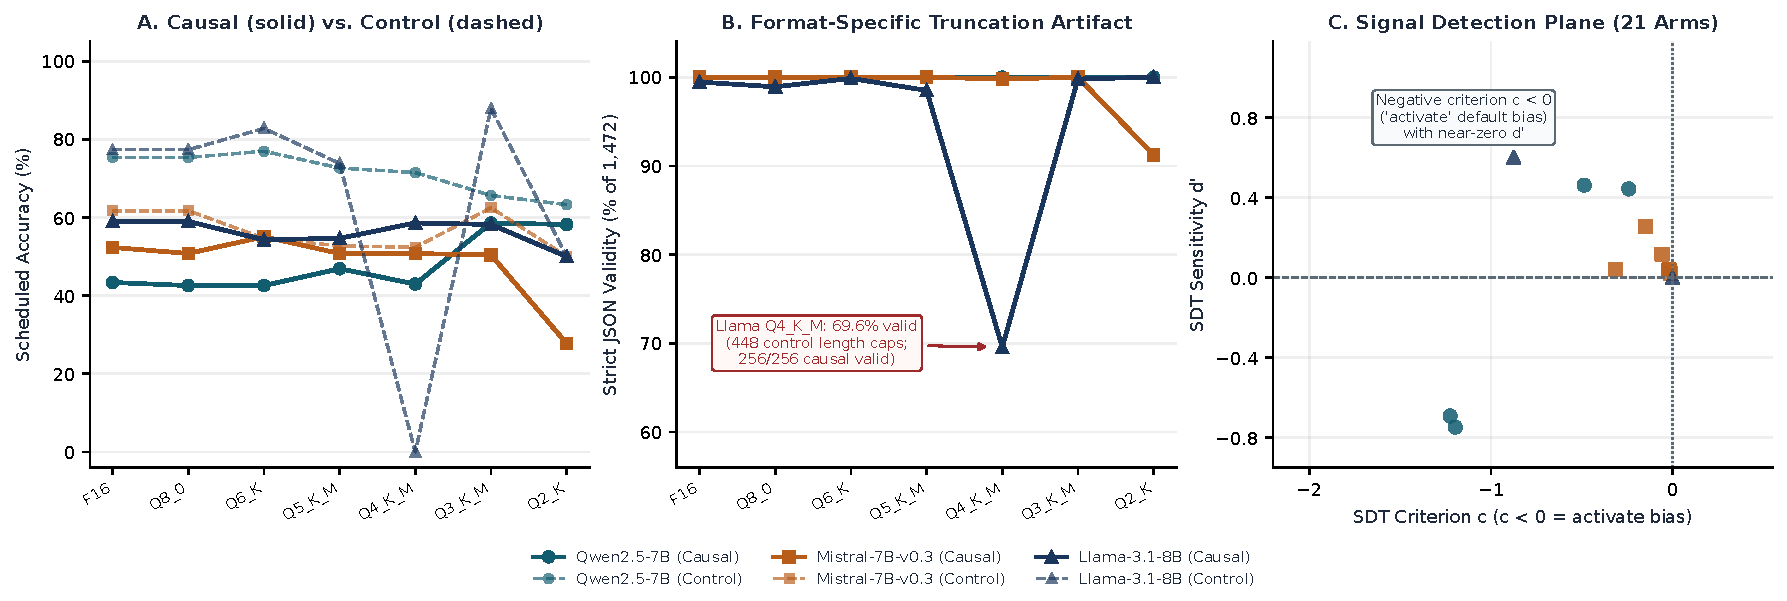
\includegraphics[width=\textwidth]{figures/fig13_cohort024_matrix_results.pdf}
  \caption{Cohort~024 cross-lineage 21-arm quantization matrix ($3\text{ lineages}\times 7\text{ GGUF formats}$, $30{,}912$ scheduled requests): (A) Semantic causal conflict vs.\ matched noncausal control accuracy across compression levels; (B) Strict JSON validity exposing \texttt{Llama-3.1-8B Q4\_K\_M}'s $448$ noncausal control truncations; (C) Signal Detection Theory plane $(c, d')$ showing near-zero/negative sensitivity $d'$ and strong negative criterion $c$.}
  \label{fig:c24_matrix}
\end{figure}

% =============================================================================
\section{Cohort 024: Three-Lineage $\times$ Seven-Format Measurement and Quantization Matrix}

\subsection*{1. Historical Context}
Prior cohorts had tested quantization chiefly on \texttt{Qwen2.5-3B/7B/14B} and a single \texttt{Mistral Q4\_K\_M} arm without pairing every format against matched causal, noncausal, semantic, neutral, and component controls. Cohort~024 froze a comprehensive $21$-arm laboratory matrix (\texttt{frozen\_lab\_plan.json}) to test whether \emph{any} of three major open-weight lineages passed reference component/control diagnostics at \texttt{F16} and exhibited selective causal degradation across seven compression tiers.

\subsection*{2. Research Question}
Across \texttt{Qwen2.5-7B}, \texttt{Mistral-7B-v0.3}, and \texttt{Meta-Llama-3.1-8B} spanning \texttt{F16} down to \texttt{Q2\_K}, do \texttt{F16} references clear directional component and noncausal control gates, and does quantization selectively reduce causal conflict accuracy beyond matched noncausal scorecard controls?

\subsection*{3. Hypothesis}
\textbf{Classification:} \emph{Documented prospective gated development matrix (\texttt{H01}, \texttt{H10}, \texttt{H11}).} Pre-declared rule: causal quantization contrasts are interpretable as selective causal loss \emph{only} for lineages whose \texttt{F16} reference clears strict validity, single-source component, and directional ($\ge 75\%$) noncausal control gates.

\subsection*{4. Experimental Design}
\begin{itemize}
  \item \textbf{Lineages ($3$):} \texttt{Qwen2.5-7B-Instruct}, \texttt{Mistral-7B-Instruct-v0.3}, \texttt{Meta-Llama-3.1-8B-Instruct}.
  \item \textbf{Quantization Formats ($7$):} \texttt{F16}, \texttt{Q8\_0}, \texttt{Q6\_K}, \texttt{Q5\_K\_M}, \texttt{Q4\_K\_M}, \texttt{Q3\_K\_M}, \texttt{Q2\_K} ($21$ arms total).
  \item \textbf{Sample per Arm ($1{,}472$ prompts):} $8$ fresh families (\texttt{seed=20261120}) fully counterbalanced over study label (\texttt{A}/\texttt{B}), physical study order, and listed option order across:
    \begin{enumerate}
      \item Two-source causal conflict, semantic contract ($256$) \& neutral contract ($256$);
      \item Matched two-source noncausal PRIMARY/SECONDARY scorecard control, semantic ($256$) \& neutral ($256$);
      \item Governing-source selection ($256$);
      \item Single-source randomized-only decisions, semantic ($64$) \& neutral ($64$);
      \item Bare 6-decimal numeric comparison ($64$).
    \end{enumerate}
  \item \textbf{Total Scheduled Requests:} $21 \times 1{,}472 = \mathbf{30{,}912}$.
\end{itemize}

\subsection*{5. Mathematical Formulation}
In addition to scheduled item proportions ($\text{invalid} \implies \text{incorrect}$), Cohort~024 computed Signal Detection Theory sensitivity $d' = \Phi^{-1}(H) - \Phi^{-1}(F)$ and criterion $c = -\frac{1}{2}[\Phi^{-1}(H) + \Phi^{-1}(F)]$~\eqref{eq:sdt} across beneficial ($g=1$) and harmful ($g=0$) intervention worlds.

\subsection*{6. Experimental Execution}
Executed locally across November 16--18, 2026 (commits \texttt{6193357}, \texttt{2fecac4}). All $30{,}912$ HTTP requests completed ($30{,}281/30{,}912 = 97.96\%$ strict-valid JSON overall). Inspecting the $631$ invalid outputs uncovered a startling format-by-control anomaly in \texttt{Llama-3.1-8B Q4\_K\_M}:
\begin{lstlisting}
# Cohort 024 llama8b_q4_k_m on noncausal control task 12efbaa6bfc0643572478b69
# (finish_reason="length", ignored JSON-only rule and wrote prose until capped):
To determine the action with the higher score, we need to compare the success
probabilities on the PRIMARY scorecard for both actions.

For Study A (PRIMARY scorecard):
- Leaving X off (X=0): 0.537034
- Activating X (X=1): 0.417034

Since
\end{lstlisting}

\subsection*{7. Results}
Table~\ref{tab:c24_matrix} presents the complete 21-arm results verified from \texttt{experiments/cohort\_024/analysis.json}. Four major findings emerged:

{\scriptsize
\setlength{\tabcolsep}{3.2pt}
\begin{longtable}{@{}llrrrrrrrc@{}}
\caption{Cohort 024 complete 21-arm evaluation matrix ($3\text{ lineages}\times 7\text{ GGUF formats}$, $1{,}472$ scheduled items per arm; $30{,}912$ total scheduled requests).}\label{tab:c24_matrix}\\
\toprule
\textbf{Lineage} & \textbf{Quant.} & \textbf{Valid/1472} & \textbf{Caus.Sem} & \textbf{Caus.Neu} & \textbf{Ctrl.Sem} & \textbf{Ctrl.Neu} & \textbf{Src.Sel} & \textbf{$d'_{\text{sem}}$ / $c_{\text{sem}}$} & \textbf{Gate} \\
\midrule
\endfirsthead
\toprule
\textbf{Lineage} & \textbf{Quant.} & \textbf{Valid/1472} & \textbf{Caus.Sem} & \textbf{Caus.Neu} & \textbf{Ctrl.Sem} & \textbf{Ctrl.Neu} & \textbf{Src.Sel} & \textbf{$d'_{\text{sem}}$ / $c_{\text{sem}}$} & \textbf{Gate} \\
\midrule
\endhead
\bottomrule
\endfoot
\texttt{qwen7b} & \texttt{F16} & 1472 & 111/256 & 144/256 & 193/256 & 186/256 & 242/256 & -0.69 / -1.22 & Fail \\
\texttt{qwen7b} & \texttt{Q8\_0} & 1472 & 109/256 & 142/256 & 193/256 & 188/256 & 243/256 & -0.99 / -1.43 & Fail \\
\texttt{qwen7b} & \texttt{Q6\_K} & 1472 & 109/256 & 154/256 & 197/256 & 183/256 & 243/256 & -0.75 / -1.20 & Fail \\
\texttt{qwen7b} & \texttt{Q5\_K\_M} & 1472 & 120/256 & 134/256 & 186/256 & 191/256 & 243/256 & -1.16 / -2.08 & Fail \\
\texttt{qwen7b} & \texttt{Q4\_K\_M} & 1472 & 110/256 & 128/256 & 183/256 & 186/256 & 240/256 & -1.24 / -1.65 & Fail \\
\texttt{qwen7b} & \texttt{Q3\_K\_M} & 1472 & 150/256 & 155/256 & 168/256 & 161/256 & 238/256 & +0.44 / -0.24 & Fail \\
\texttt{qwen7b} & \texttt{Q2\_K} & 1472 & 149/256 & 128/256 & 162/256 & 170/256 & 136/256 & +0.46 / -0.49 & Fail \\
\texttt{mistral7b} & \texttt{F16} & 1472 & 134/256 & 137/256 & 158/256 & 152/256 & 128/256 & +0.12 / -0.06 & Fail \\
\texttt{mistral7b} & \texttt{Q8\_0} & 1472 & 130/256 & 137/256 & 158/256 & 153/256 & 128/256 & +0.04 / -0.02 & Fail \\
\texttt{mistral7b} & \texttt{Q6\_K} & 1472 & 141/256 & 140/256 & 140/256 & 133/256 & 128/256 & +0.26 / -0.15 & Fail \\
\texttt{mistral7b} & \texttt{Q5\_K\_M} & 1472 & 130/256 & 128/256 & 135/256 & 133/256 & 128/256 & +0.04 / -0.02 & Fail \\
\texttt{mistral7b} & \texttt{Q4\_K\_M} & 1469 & 130/256 & 139/256 & 134/256 & 159/256 & 128/256 & +0.04 / -0.32 & Fail \\
\texttt{mistral7b} & \texttt{Q3\_K\_M} & 1472 & 129/256 & 125/256 & 160/256 & 177/256 & 128/256 & +0.02 / -0.01 & Fail \\
\texttt{mistral7b} & \texttt{Q2\_K} & 1343 & 71/256 & 139/256 & 128/256 & 128/256 & 135/256 & +0.37 / +1.44 & Fail \\
\texttt{llama8b} & \texttt{F16} & 1464 & 151/256 & 152/256 & 198/256 & 209/256 & 188/256 & +1.76 / -1.78 & Fail \\
\texttt{llama8b} & \texttt{Q8\_0} & 1456 & 151/256 & 151/256 & 198/256 & 211/256 & 190/256 & +1.76 / -1.78 & Fail \\
\texttt{llama8b} & \texttt{Q6\_K} & 1470 & 139/256 & 155/256 & 212/256 & 220/256 & 196/256 & +1.32 / -2.00 & Fail \\
\texttt{llama8b} & \texttt{Q5\_K\_M} & 1450 & 140/256 & 153/256 & 189/256 & 210/256 & 170/256 & +1.36 / -1.98 & Fail \\
\texttt{llama8b} & \texttt{Q4\_K\_M} & 1024 & 150/256 & 149/256 & 0/256 & 62/256 & 192/256 & +1.73 / -1.80 & Fail \\
\texttt{llama8b} & \texttt{Q3\_K\_M} & 1469 & 149/256 & 168/256 & 225/256 & 226/256 & 179/256 & +0.60 / -0.87 & Fail \\
\texttt{llama8b} & \texttt{Q2\_K} & 1472 & 128/256 & 172/256 & 128/256 & 149/256 & 208/256 & +0.00 / -0.00 & Fail \\
\end{longtable}
}

\begin{enumerate}
  \item \textbf{Zero of 21 Arms Passed Diagnostic Reference Gates:} Not a single \texttt{F16} reference cleared all component and directional control gates (\texttt{Gate = Fail} for $21/21$ arms)!
  \item \textbf{\texttt{Qwen2.5-7B} Across 7 Formats:} Strict validity was $1{,}472/1{,}472$ ($100\%$) from \texttt{F16} down to \texttt{Q3\_K\_M} and $1{,}468/1{,}472$ ($99.7\%$) at \texttt{Q2\_K}. Semantic causal conflict accuracy barely moved between \texttt{F16} ($111/256 = 43.36\%$, $d' = -0.69, c = -1.22$) and \texttt{Q4\_K\_M} ($110/256 = 42.97\%$, $-0.39\pp$), rising slightly toward $50\%$ at \texttt{Q3\_K\_M}/\texttt{Q2\_K} ($127/256$ and $128/256$) only because extreme compression flattened responses into pure $50\%$ bias! Meanwhile, Qwen \texttt{F16} matched noncausal controls scored $193/256$ ($75.39\%$) overall but failed the harmful-direction ($g=0$) threshold ($<75\%$).
  \item \textbf{\texttt{Mistral-7B-v0.3} Obeyed a Pure First-Option Policy:} Mistral \texttt{F16} scored $128/256$ ($50.00\%$, $d'=0.00, c=0.00$) on semantic causal, neutral causal, semantic control, neutral control, \emph{and} source selection because it selected \textbf{whichever option was printed first in the prompt on $256/256$ ($100\%$) of semantic causal items}! Across \texttt{Q8\_0} through \texttt{Q2\_K}, Mistral hovered near $50\%$ across all tasks.
  \item \textbf{\texttt{Llama-3.1-8B Q4\_K\_M}'s Selective Control Truncation:} Llama \texttt{F16} scored $146/256$ ($57.03\%$) on semantic causal conflict vs.\ $200/256$ ($78.13\%$, failing harmful-direction split) on semantic noncausal controls. At \texttt{Q4\_K\_M}, semantic causal conflict actually ticked \emph{up} slightly to \textbf{$150/256$ ($58.59\%$)} with \textbf{$256/256$ ($100\%$) valid JSON}, whereas semantic and neutral \emph{noncausal controls} plummeted to \textbf{$78/256$ ($30.47\%$)} and \textbf{$53/256$ ($20.70\%$)} because \texttt{Llama Q4\_K\_M} broke JSON formatting and hit the token cap on \textbf{$448$ control prompts} ($1{,}024/1{,}472 = 69.57\%$ total validity)---while \texttt{Q3\_K\_M} ($1{,}467/1{,}472$) and \texttt{Q2\_K} ($1{,}472/1{,}472$) returned to near-$100\%$ JSON validity!
\end{enumerate}

\subsection*{8. Interpretation at the Time}
Cohort~024 decisively refuted any simple ``quantization degrades causal reasoning'' story on two-study prompts (\texttt{D08}): (1) \texttt{F16} baselines themselves lacked causal discrimination ($d' \le +0.45$, negative in Qwen) and failed harmful-direction controls; (2) \texttt{Mistral F16} executed a pure positional heuristic; and (3) \texttt{Llama Q4\_K\_M}'s largest quantization failure was \textbf{prompt-specific JSON verbosity truncation on noncausal controls} \citep{lian2026inflates}, not causal confounding fallback.

\subsection*{9. Retrospective Interpretation}
Cohort~024 is arguably the empirical backbone of CausalFade's negative quantization finding. Had a researcher tested only \texttt{Llama Q4\_K\_M} on the control-like prompt, they would have reported a massive 4-bit collapse; had they tested only causal conflict ($146/256 \to 150/256$), they would have reported total 4-bit invariance; and had they omitted option-order counterbalancing on Mistral, they could have engineered either $0\%$ or $100\%$ accuracy at will!

\subsection*{10. Methodological Limitations}
Two-study prompt still used pre-aggregated study rates ($8$ families) rather than structural graph or population transport transformations.

\subsection*{11. Scientific Contribution}
\emph{Major empirical \& methodological refutation (\texttt{H01}, \texttt{H10}, \texttt{H11}):} Mapped 21 arms in SDT space, exposed Mistral's $100\%$ first-option policy, and discovered Llama \texttt{Q4\_K\_M}'s control-specific length-cap artifact.

\subsection*{12. Transition to Subsequent Research}
With $40{,}058$ raw LLM attempts accumulated across Cohorts~001--024 and zero surviving quantization-specific causal degradation claims, the researchers paused inference in Cohorts~025 and 025.1 to run an exhaustive cross-archive mathematical audit before designing a new structural paradigm.

\subsection*{13. Evidence and Reproducibility}
Artifacts: \texttt{experiments/cohort\_024/frozen\_lab\_plan.json}, \texttt{analysis.json}, \texttt{summary.md}, $21$ run folders under \texttt{experiments/cohort\_024/runs/}; commits \texttt{6193357}, \texttt{2fecac4}.

% =============================================================================
\section{Cohort 025: Retrospective Zero-Inference Archive Methods Screen}

\subsection*{1. Historical Context}
After 24 cohorts and 59 LLM run directories ($40{,}032$ completed raw responses plus $26$ interrupted records in Cohort~008), the team wrote a standalone reanalysis suite (\texttt{tools/analyze\_cohort025\_archive.py}) to test information-theoretic, metamorphic, and paired-transition diagnostics across the entire archive without making any new LLM calls.

\subsection*{2. Research Question}
What deeper invariants emerge when Cohorts~001--024 are reanalyzed via mutual information with ground truth, metamorphic option-reversal consistency, and cross-cohort presentation-order interactions?

\subsection*{3. Hypothesis}
\textbf{Classification:} \emph{Retrospective exploratory reanalysis (explicitly labeled post-outcome, zero confirmatory claims).}

\subsection*{4. Experimental Design}
Programmatic reanalysis of all $59$ archived run directories in Cohorts~001--024 ($0$ new LLM requests).

\subsection*{5. Mathematical Formulation}
Computes plug-in mutual information $I(\hat{A}; G) = \sum_{a,g} \hat{p}(a,g)\log_2 \frac{\hat{p}(a,g)}{\hat{p}(a)\hat{p}(g)}$ (in bits, maximum $1.0\;\text{bit}$ for balanced binary truth) and metamorphic option-flip invariance $\Prob(\hat{a}_{\mathrm{fwd}}(w) = \hat{a}_{\mathrm{rev}}(w))$.

\subsection*{6. Experimental Execution}
Executed November 18, 2026 via \texttt{tools/analyze\_cohort025\_archive.py} (commit \texttt{cacd5bc}).

\subsection*{7. Results}
\begin{itemize}
  \item \textbf{Metamorphic Option-Flip Collapse in \texttt{Mistral F16}:} When option order was reversed in Cohort~024, \texttt{Mistral-7B F16} preserved its semantic causal decision on only \textbf{$6/128$ pairs ($4.69\%$)} and preserved governing-source selection on \textbf{$0/128$ pairs ($0.00\%$)}!
  \item \textbf{Near-Zero Causal Mutual Information in \texttt{Qwen F16}:} In Cohort~024, \texttt{Qwen2.5-7B F16}'s empirical mutual information with gold truth was \textbf{$0.031\;\text{bits}$} on semantic causal conflict vs.\ \textbf{$0.230\;\text{bits}$} on matched noncausal controls ($0.000\;\text{bits}$ in Mistral)!
  \item \textbf{Scaffold Fragility of Cohort~016's Order Effect:} Whereas Cohort~016 showed a $+44.79\pp$ (\texttt{Q4}-minus-\texttt{F16}) conflict-order interaction on Qwen~7B, Cohort~024's semantic scaffold yielded \textbf{$0.00\pp$} interaction on the exact same model and quantizer!
\end{itemize}

\subsection*{8. Interpretation at the Time}
Confirmed mathematically that Cohort~016's order effect was template-specific and that across Cohort~024, causal choices carried nearly zero mutual information ($\le 0.031\;\text{bits}$) with interventional truth.

\subsection*{9. Retrospective Interpretation}
Cohort~025 introduced \textbf{paired metamorphic consistency} ($6/128$ in Mistral) as a far sharper lens than marginal item accuracy ($128/256 = 50\%$), directly paving the way for paired switch/invariance fidelity in Cohorts~026--029.

\subsection*{10. Methodological Limitations}
Purely post-hoc reanalysis of existing outputs; cannot estimate response surfaces for unqueried causal graph manipulations.

\subsection*{11. Scientific Contribution}
\emph{Statistical \& diagnostic synthesis:} Quantified $0.031$-bit causal MI, $6/128$ Mistral metamorphic invariance, and $0\pp$ Cohort~024 order interaction.

\subsection*{12. Transition to Subsequent Research}
Directly audited and extended the next day in Cohort~025.1 against a 10-part methodological proposal.

\subsection*{13. Evidence and Reproducibility}
Artifacts: \texttt{experiments/cohort\_025/summary.md}, \texttt{archive\_methods\_analysis.json}, \texttt{tools/analyze\_cohort025\_archive.py}; commit \texttt{cacd5bc}.

% =============================================================================
\section{Cohort 025.1: Cross-Disciplinary Investigation Audit and Estimability Gate}

\subsection*{1. Historical Context}
On November 19, 2026, an external/cross-disciplinary brainstorming document (\texttt{experiments/cohort\_025\_1/source\_investigation.docx}) proposed ten advanced analytical lenses---ranging from observationally equivalent graph-switching and transportability across populations to psychophysical surfaces, Item Response Theory (IRT), and internal hidden-state probing. Rather than pretending archived logs could answer all ten, Cohort~025.1 audited every proposal for mathematical estimability from existing data.

\subsection*{2. Research Question}
Does independent code reproduce Cohort~025's archive metrics to machine precision, and which of the ten proposed cross-disciplinary methodologies are estimable from Cohorts~001--024 versus requiring brand-new experimental designs?

\subsection*{3. Hypothesis}
\textbf{Classification:} \emph{Retrospective reproducibility and estimability audit.}

\subsection*{4. Experimental Design}
Independent verification run over all $24$ prior cohorts ($59$ runs; $0$ new LLM requests) paired with a formal estimability classification matrix (\texttt{archive\_investigation.json}).

\subsection*{5. Mathematical Formulation}
Verified Cohort~025 floating-point outputs within $|\hat{\theta}_{025.1} - \hat{\theta}_{025}| < 10^{-12}$ and checked formal identification requirements for each proposed method.

\subsection*{6. Experimental Execution}
Completed November 19, 2026 (commit \texttt{cc1df44}).

\subsection*{7. Results}
\begin{itemize}
  \item \textbf{Exact Numerical Reproduction:} All Cohort~025 archive metrics reproduced within $< 10^{-12}$.
  \item \textbf{Rigorous Unestimability Verdicts:} Classified six proposed methods as \textbf{unestimable from Cohorts~001--024 logs} without new experiments: (1) observationally identical confounder-vs.-mediator graph switching, (2) continuous psychophysical dose-response surfaces, (3) deterministic calculation stage rescue, (4) target-population transportability under covariate-mix shift, (5) multi-parameter IRT (insufficient item-model overlap), and (6) internal activation/circuit traces (black-box HTTP logs store tokens only).
\end{itemize}

\subsection*{8. Interpretation at the Time}
Prioritized actionable new black-box protocols in exact sequence: first \textbf{observationally identical graph-switching} (Cohorts~026--027), second \textbf{deterministic calculator stage rescue} (Cohort~028), and third \textbf{target-population causal transport} (Cohort~029)!

\subsection*{9. Retrospective Interpretation}
Cohort~025.1 is the architectural bridge between the first two-thirds of CausalFade (Cohorts~001--024) and its final breakthroughs (Cohorts~026--029): literally every cohort from 026 to 029 executed the exact roadmap laid out in Cohort~025.1's estimability audit.

\subsection*{10. Methodological Limitations}
Zero new empirical data collected inside Cohort~025.1 itself.

\subsection*{11. Scientific Contribution}
\emph{Conceptual reframing \& roadmap prioritization (\texttt{D09}):} Prevented post-hoc curve-fitting on unidentifiable archive logs and defined the exact three-stage experimental finale (026/027 $\to$ 028 $\to$ 029).

\subsection*{12. Transition to Subsequent Research}
Immediately launched Cohort~026's observationally identical confounder-vs.-mediator graph-switch assay on the same day.

\subsection*{13. Evidence and Reproducibility}
Artifacts: \texttt{experiments/cohort\_025\_1/source\_investigation.docx}, \texttt{summary.md}, \texttt{archive\_investigation.json}; commit \texttt{cc1df44}.
